\documentclass[a4paper]{article}

\def\npart {IB}
\def\nterm {Michaelmas}
\def\nyear {2015}
\def\nlecturer {J. M. Evans}
\def\ncourse {Quantum Mechanics}
\def\nnotready {}

% Imports
\ifx \nextra \undefined
  \usepackage[pdftex,
    hidelinks,
    pdfauthor={Dexter Chua},
    pdfsubject={Cambridge Maths Notes: Part \npart\ - \ncourse},
    pdftitle={Part \npart\ - \ncourse},
  pdfkeywords={Cambridge Mathematics Maths Math \npart\ \nterm\ \nyear\ \ncourse}]{hyperref}
  \title{Part \npart\ - \ncourse}
\else
  \usepackage[pdftex,
    hidelinks,
    pdfauthor={Dexter Chua},
    pdfsubject={Cambridge Maths Notes: Part \npart\ - \ncourse\ (\nextra)},
    pdftitle={Part \npart\ - \ncourse\ (\nextra)},
  pdfkeywords={Cambridge Mathematics Maths Math \npart\ \nterm\ \nyear\ \ncourse\ \nextra}]{hyperref}

  \title{Part \npart\ - \ncourse \\ {\Large \nextra}}
\fi

\author{Lectured by \nlecturer \\\small Notes taken by Dexter Chua}
\date{\nterm\ \nyear}

\usepackage{alltt}
\usepackage{amsfonts}
\usepackage{amsmath}
\usepackage{amssymb}
\usepackage{amsthm}
\usepackage{booktabs}
\usepackage{caption}
\usepackage{enumitem}
\usepackage{fancyhdr}
\usepackage{graphicx}
\usepackage{mathtools}
\usepackage{microtype}
\usepackage{multirow}
\usepackage{pdflscape}
\usepackage{pgfplots}
\usepackage{siunitx}
\usepackage{tabularx}
\usepackage{tikz}
\usepackage{tkz-euclide}
\usepackage[normalem]{ulem}
\usepackage[all]{xy}

\pgfplotsset{compat=1.12}

\pagestyle{fancyplain}
\lhead{\emph{\nouppercase{\leftmark}}}
\ifx \nextra \undefined
  \rhead{
    \ifnum\thepage=1
    \else
      \npart\ \ncourse
    \fi}
\else
  \rhead{
    \ifnum\thepage=1
    \else
      \npart\ \ncourse\ (\nextra)
    \fi}
\fi
\usetikzlibrary{arrows}
\usetikzlibrary{decorations.markings}
\usetikzlibrary{decorations.pathmorphing}
\usetikzlibrary{positioning}
\usetikzlibrary{fadings}
\usetikzlibrary{intersections}
\usetikzlibrary{cd}

\newcommand*{\Cdot}{\raisebox{-0.25ex}{\scalebox{1.5}{$\cdot$}}}
\newcommand {\pd}[2][ ]{
  \ifx #1 { }
    \frac{\partial}{\partial #2}
  \else
    \frac{\partial^{#1}}{\partial #2^{#1}}
  \fi
}

% Theorems
\theoremstyle{definition}
\newtheorem*{aim}{Aim}
\newtheorem*{axiom}{Axiom}
\newtheorem*{claim}{Claim}
\newtheorem*{cor}{Corollary}
\newtheorem*{defi}{Definition}
\newtheorem*{eg}{Example}
\newtheorem*{fact}{Fact}
\newtheorem*{law}{Law}
\newtheorem*{lemma}{Lemma}
\newtheorem*{notation}{Notation}
\newtheorem*{prop}{Proposition}
\newtheorem*{thm}{Theorem}

\renewcommand{\labelitemi}{--}
\renewcommand{\labelitemii}{$\circ$}
\renewcommand{\labelenumi}{(\roman{*})}

\let\stdsection\section
\renewcommand\section{\newpage\stdsection}

% Strike through
\def\st{\bgroup \ULdepth=-.55ex \ULset}

% Maths symbols
\newcommand{\bra}{\langle}
\newcommand{\ket}{\rangle}

\newcommand{\N}{\mathbb{N}}
\newcommand{\Z}{\mathbb{Z}}
\newcommand{\Q}{\mathbb{Q}}
\renewcommand{\H}{\mathbb{H}}
\newcommand{\R}{\mathbb{R}}
\newcommand{\C}{\mathbb{C}}
\newcommand{\Prob}{\mathbb{P}}
\renewcommand{\P}{\mathbb{P}}
\newcommand{\E}{\mathbb{E}}
\newcommand{\F}{\mathbb{F}}
\newcommand{\cU}{\mathcal{U}}
\newcommand{\RP}{\mathbb{RP}}
\newcommand{\CP}{\mathbb{CP}}

\newcommand{\ph}{\,\cdot\,}

\DeclareMathOperator{\sech}{sech}
\DeclareMathOperator{\cosech}{cosech}
\DeclareMathOperator{\cosec}{cosec}

\DeclareMathOperator{\covol}{covol}
\DeclareMathOperator{\vol}{vol}

\let\Im\relax
\let\Re\relax
\DeclareMathOperator{\Im}{Im}
\DeclareMathOperator{\Re}{Re}
\DeclareMathOperator{\im}{im}
\DeclareMathOperator{\image}{image}
\DeclareMathOperator{\Ann}{Ann}

\DeclareMathOperator*{\res}{res}
\DeclareMathOperator{\Res}{Res}
\DeclareMathOperator{\Ind}{Ind}

\DeclareMathOperator{\tr}{tr}
\DeclareMathOperator{\diag}{diag}
\DeclareMathOperator{\rank}{rank}
\DeclareMathOperator{\card}{card}
\DeclareMathOperator{\spn}{span}
\DeclareMathOperator{\adj}{adj}

\DeclareMathOperator{\erf}{erf}
\DeclareMathOperator{\erfc}{erfc}

\DeclareMathOperator{\ord}{ord}
\DeclareMathOperator{\Sym}{Sym}

\DeclareMathOperator{\sgn}{sgn}
\DeclareMathOperator{\orb}{orb}
\DeclareMathOperator{\stab}{stab}
\DeclareMathOperator{\ccl}{ccl}

\DeclareMathOperator{\lcm}{lcm}
\DeclareMathOperator{\hcf}{hcf}

\DeclareMathOperator{\Int}{Int}
\DeclareMathOperator{\id}{id}

\DeclareMathOperator{\betaD}{beta}
\DeclareMathOperator{\gammaD}{gamma}
\DeclareMathOperator{\Poisson}{Poisson}
\DeclareMathOperator{\binomial}{binomial}
\DeclareMathOperator{\multinomial}{multinomial}
\DeclareMathOperator{\Bernoulli}{Bernoulli}
\DeclareMathOperator{\like}{like}

\DeclareMathOperator{\var}{var}
\DeclareMathOperator{\cov}{cov}
\DeclareMathOperator{\bias}{bias}
\DeclareMathOperator{\mse}{mse}
\DeclareMathOperator{\corr}{corr}

\DeclareMathOperator{\otp}{otp}
\DeclareMathOperator{\dom}{dom}

\DeclareMathOperator{\Root}{Root}
\DeclareMathOperator{\supp}{supp}
\DeclareMathOperator{\rel}{rel}
\DeclareMathOperator{\Hom}{Hom}
\DeclareMathOperator{\Aut}{Aut}
\DeclareMathOperator{\Gal}{Gal}
\DeclareMathOperator{\Mat}{Mat}
\DeclareMathOperator{\End}{End}
\DeclareMathOperator{\Char}{char}
\DeclareMathOperator{\ev}{ev}
\DeclareMathOperator{\St}{St}
\DeclareMathOperator{\Lk}{Lk}
\DeclareMathOperator{\disc}{disc}
\DeclareMathOperator{\Isom}{Isom}
\DeclareMathOperator{\length}{length}
\DeclareMathOperator{\energy}{energy}
\DeclareMathOperator{\area}{area}
\DeclareMathOperator{\Syl}{Syl}
\DeclareMathOperator{\cl}{cl}
\DeclareMathOperator{\fix}{fix}

\newcommand{\GL}{\mathrm{GL}}
\newcommand{\SL}{\mathrm{SL}}
\newcommand{\PGL}{\mathrm{PGL}}
\newcommand{\PSL}{\mathrm{PSL}}
\newcommand{\PSU}{\mathrm{PSU}}
\newcommand{\Or}{\mathrm{O}}
\newcommand{\SO}{\mathrm{SO}}
\newcommand{\U}{\mathrm{U}}
\newcommand{\SU}{\mathrm{SU}}

\renewcommand{\d}{\mathrm{d}}
\newcommand{\D}{\mathrm{D}}

\tikzset{->/.style = {decoration={markings,
                                  mark=at position 1 with {\arrow[scale=2]{latex'}}},
                      postaction={decorate}}}
\tikzset{<-/.style = {decoration={markings,
                                  mark=at position 0 with {\arrowreversed[scale=2]{latex'}}},
                      postaction={decorate}}}
\tikzset{<->/.style = {decoration={markings,
                                   mark=at position 0 with {\arrowreversed[scale=2]{latex'}},
                                   mark=at position 1 with {\arrow[scale=2]{latex'}}},
                       postaction={decorate}}}
\tikzset{->-/.style = {decoration={markings,
                                   mark=at position #1 with {\arrow[scale=2]{latex'}}},
                       postaction={decorate}}}
\tikzset{-<-/.style = {decoration={markings,
                                   mark=at position #1 with {\arrowreversed[scale=2]{latex'}}},
                       postaction={decorate}}}

\tikzset{circ/.style = {fill, circle, inner sep = 0, minimum size = 3}}
\tikzset{mstate/.style={circle, draw, blue, text=black, minimum width=0.7cm}}

\definecolor{mblue}{rgb}{0.2, 0.3, 0.8}
\definecolor{morange}{rgb}{1, 0.5, 0}
\definecolor{mgreen}{rgb}{0.1, 0.4, 0.2}
\definecolor{mred}{rgb}{0.5, 0, 0}

\def\drawcirculararc(#1,#2)(#3,#4)(#5,#6){%
    \pgfmathsetmacro\cA{(#1*#1+#2*#2-#3*#3-#4*#4)/2}%
    \pgfmathsetmacro\cB{(#1*#1+#2*#2-#5*#5-#6*#6)/2}%
    \pgfmathsetmacro\cy{(\cB*(#1-#3)-\cA*(#1-#5))/%
                        ((#2-#6)*(#1-#3)-(#2-#4)*(#1-#5))}%
    \pgfmathsetmacro\cx{(\cA-\cy*(#2-#4))/(#1-#3)}%
    \pgfmathsetmacro\cr{sqrt((#1-\cx)*(#1-\cx)+(#2-\cy)*(#2-\cy))}%
    \pgfmathsetmacro\cA{atan2(#2-\cy,#1-\cx)}%
    \pgfmathsetmacro\cB{atan2(#6-\cy,#5-\cx)}%
    \pgfmathparse{\cB<\cA}%
    \ifnum\pgfmathresult=1
        \pgfmathsetmacro\cB{\cB+360}%
    \fi
    \draw (#1,#2) arc (\cA:\cB:\cr);%
}
\newcommand\getCoord[3]{\newdimen{#1}\newdimen{#2}\pgfextractx{#1}{\pgfpointanchor{#3}{center}}\pgfextracty{#2}{\pgfpointanchor{#3}{center}}}

\def\Xint#1{\mathchoice
   {\XXint\displaystyle\textstyle{#1}}%
   {\XXint\textstyle\scriptstyle{#1}}%
   {\XXint\scriptstyle\scriptscriptstyle{#1}}%
   {\XXint\scriptscriptstyle\scriptscriptstyle{#1}}%
   \!\int}
\def\XXint#1#2#3{{\setbox0=\hbox{$#1{#2#3}{\int}$}
     \vcenter{\hbox{$#2#3$}}\kern-.5\wd0}}
\def\ddashint{\Xint=}
\def\dashint{\Xint-}


\begin{document}
\maketitle
{\small
\noindent\textbf{Physical background}\\
Photoelectric effect. Electrons in atoms and line spectra. Particle diffraction.\hspace*{\fill} [1]

\vspace{10pt}
\noindent\textbf{Schr\"odinger equation and solutions}\\
De Broglie waves. Schr\"odinger equation. Superposition principle. Probability interpretation, density and current.\hspace*{\fill} [2]

\vspace{5pt}
\noindent Stationary states. Free particle, Gaussian wave packet. Motion in 1-dimensional potentials, parity. Potential step, square well and barrier. Harmonic oscillator.\hspace*{\fill} [4]

\vspace{10pt}
\noindent\textbf{Observables and expectation values}\\
Position and momentum operators and expectation values. Canonical commutation relations. Uncertainty principle.\hspace*{\fill} [2]

\vspace{5pt}
\noindent Observables and Hermitian operators. Eigenvalues and eigenfunctions. Formula for expectation value.\hspace*{\fill} [2]

\vspace{10pt}
\noindent\textbf{Hydrogen atom}\\
Spherically symmetric wave functions for spherical well and hydrogen atom.

\vspace{5pt}
\noindent Orbital angular momentum operators. General solution of hydrogen atom.\hspace*{\fill} [5]
}

\tableofcontents
\setcounter{section}{-1}
\section{Introduction}
Quantum mechanics (QM) is a radical generalization of classical physics. Profound new features of quantum mechanics include
\begin{enumerate}
  \item \emph{Quantisation} - Quantities such as energy are often restricted to a discrete set of values, or appear in definite amounts , called \emph{quanta}.
  \item \emph{Wave-particle duality} - Classical concepts of particles and waves become merged in quantum mechanics. They are different aspects of a single entity. So an electron will no longer be thought of a ``particle'' but an entity that has properties of both particles and waves.
  \item Probability and uncertainty - Predictions in quantum mechanics involve probability in a fundamental way. This probability does not arise from our lack of knowledge of the system, but is a genuine uncertainty in reality. In particular, there are limits to what we can ask about a physical system, even in principle. For example, the Heisenberg Uncertainty Relation entails that we cannot accurately know the position \emph{and} momentum of a particle.
\end{enumerate}
Quantum mechanics also involves a new fundamental constant $h$ or $\hbar = \frac{h}{2\pi}$. The dimension of this is $[h] = ML^2T^{-1} = [\text{energy}]\times [\text{time}] = [\text{position}] \times [\text{momentum}]$.

We can think of this constant as representing the ``strength'' of quantum effects. Despite having these new profound features, we expect to recover classical physics when we take the limit $\hbar \to 0$.

Historically, there are a few experiments that led to the development of quantum mechanics.
\subsection{Light quanta}
In quantum mechanics, light (or electromagnetic waves) consists of quanta called photons. We can think of them as waves that come in discrete ``packets'' that behave like particles.

In particular, photons behave like particles with energy $E = h \nu = \hbar \omega$, where $\nu$ is the frequency and $\omega = 2\pi \nu$ is the angular frequency. However, we usually don't care about $\nu$ and just call $\omega$ the frequency.

Similarly, the momentum is given by $p = h/\lambda = \hbar k$, where $\lambda$ is the wavelength and $k = 2\pi/\lambda$ is the wave number.

For electromagnetic waves, the speed is $c = \omega/k = \nu\lambda$. This is consistent with the fact that photons are massless particles, since we have
\[
  E = cp,
\]
as entailed by special relativity.

Historically, Planck used the concept of quanta and the energy-frequency relation to derive the spectrum of black body of ``black-body'' radiation that is consistent with experimental results. However, they were not yet sure that light indeed come in quanta. It could have just been a mathematical trick to derive the desired result.

The physical reality of photons was clarified by Einstein in explaining the \emph{photo-electric effect}.

When we shine some light (or electromagnetic radiation $\gamma$) of frequency $\omega$ onto certain metals, this can cause an emission of electrons ($e$). We can measure the maximum kinetic energy $K$ of these electrons.
\begin{center}
  \begin{tikzpicture}
    \draw (-2, 0) -- (2, 0);
    \draw [decorate, decoration={snake}] (-2, 2) -- (0, 0) node [pos = 0.5, anchor=south west] {$\gamma$}; % make curly
    \draw [->] (0, 0) -- (2, 2) node [right] {$e$};
  \end{tikzpicture}
\end{center}
Experiments show that
\begin{enumerate}
  \item The number of electrons emitted depends on the intensity (brightness) of the light, but not the frequency.
  \item The kinetic energy $K$ depends only (linearly) on the frequency but not the intensity.
  \item For $\omega < \omega_0$ (for some critical value $\omega_0$), \emph{no} electrons are emitted at all.
\end{enumerate}
This is hard to understand classically, but is exactly as expected if each electron emitted is due to the impact with a single photon. If $W$ is the energy required to liberate an electron, then we would expect $K = \hbar \omega - W$ by the conservation of energy. We will have no emission if $\omega < \omega_0 = W/\hbar$.

\subsection{Bohr model of the atom}
When we heat atoms up to make them emit light; or shine light at atoms so that they absorb light, we will find that light is emitted and absorbed at very specific frequencies, known as the emission and absorption spectra. This suggests that the inner structure of atoms is discrete.

However, in the classical model, the simplest atom, the hydrogen, consists of an electron with charge $-e$ and mass $m$, orbiting a proton of charge $+e$ and mas $m_p \gg m$ fixed at the origin.

The potential energy is
\[
  V(r) = -\frac{e^2}{4\pi\varepsilon_0}\frac{1}{r}.
\]
This implies that the angular momentum $\mathbf{L}$ is constant, and the energy $E = \frac{1}{2}mv^2 + V(r)$ is constant.

This is not a very satisfactory model for the atom. First of all, it cannot explain the discrete emission and absorption spectra. More importantly, while this model seems like a mini solar system, electromagnetism behave differently from gravitation. To maintain a circular orbit, an acceleration has to be applied onto the electron. Indeed, the force is given by
\[
  F = \frac{mv^2}{r} = \frac{e^2}{4\pi \varepsilon_0}\frac{1}{r^2}.
\]
Accelerating particles emit radiation and lose energy. So according to classical electrodynamics, the electron will just decay into the proton and atoms will implode.

The solution to this problem is to simply declare that this cannot happen. The \emph{Bohr quantization conditions} restricts the classical orbits by saying that the angular momentum can only take values
\[
  L = mrv = n\hbar
\]
for $n = 1, 2, \cdots$. Using these, together with the force equation, we can solve $r$ and $v$ completely for each $n$and obtain
\begin{align*}
  r_n &= \frac{4\pi \varepsilon_0}{me^2}\hbar^2 n^2\\
  v_n &= \frac{e^2}{4\pi \varepsilon_0}\frac{1}{\hbar n}\\
  E_n &= -\frac{1}{2}m\left(\frac{e^2}{4\pi \varepsilon_0 \hbar}\right)^2 \frac{1}{n^2}.
\end{align*}
Now we assume that the electron can make transitions between different energy levels $n$ and $m > n$, accompanied by emission or absorption of a photon of frequency $\omega$ given by
\[
  E = \hbar \omega = E_n - E_m = \frac{1}{2}m \left(\frac{e^2}{4\pi \varepsilon_0 \hbar}\right)^2\left(\frac{1}{n^2} - \frac{1}{m^2}\right).
\]
\begin{center}
  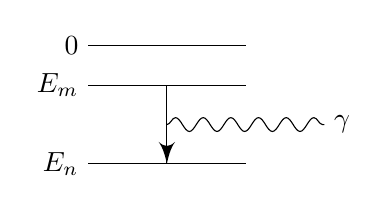
\begin{tikzpicture}
    \draw (-1, 0) node [left] {$0$} -- (1, 0);
    \draw (-1, -0.5) node [left] {$E_m$} -- (1, -0.5);
    \draw (-1, -1.5) node [left] {$E_n$} -- (1, -1.5);
    \draw [->] (0, -0.5) -- (0, -1.5);
    \draw [decorate, decoration={snake}] (0, -1) -- (2, -1) node [right] {$\gamma$};
  \end{tikzpicture}
\end{center}

\end{document}
